\chapter{Background}
There has been many efforts made to enable energy efficiency in smart-phones and in IoT in general. They are a range of solutions tried out in \emph{Hardware Architecture} level \cite{EE:MCCarch,EE:JVM}, \emph{Data communication} level \cite{EE:eTime,EE:Multinets},  \emph{Network infrastructure} level \cite{EE:Hier} and in \emph{Protocols} optimization \cite{EE:Protocol}. As Intel summed up in \cite{EE:GreenSW}, \emph{Software Energy Efficiency} is towards achieving \emph{Computational Efficiency}, \emph{Data Efficiency}, \emph{Context Awareness} and \emph{Idle Efficiency} in broader sense. Few common problems with most of the existing solutions are including: 1) system as a whole was not considered;
2) trade-off between components was not properly considered;
3) interdependences of the components was not properly studied;
4) the existing solutions are suboptimal. For measuring energy consumption, solid background has been provided  in \cite{EE:Measure}. Internet of Things-Architecture, a consortium is rigorously developing architectural reference models. The models could potentially serve the best initial  guidance towards concrete architecture for the problem of interest and eventually towards the actual system architecture \cite{IoTA:ARM}. In \cite{Orches:Arch}, devices orchestration is explained in business process point of view.


%%%%%%%%%%%%% Extra %%%%
%\begin{wrapfigure}{l}{0.3\textwidth}
% \begin{center}
%  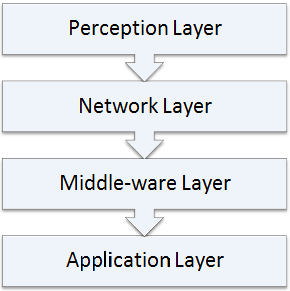
\includegraphics[scale=0.30]{Figures/IoTArch.png}
% \end{center}
% \caption{IoT Architecture}
%\end{wrapfigure}

%\begin{figure}[H]
% \begin{center}
%  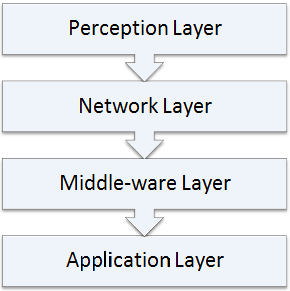
\includegraphics[scale=0.30]{Figures/IoTArch.png}
% \end{center}
% \caption{IoT Architecture}
%\end{figure}

% \cite{EE:Protocol,EE:Hier,EE:RedunData,EE:Diagnosis,
% EE:Measure,EE:MeasureWiFi,EE:Perform,EE:GreenSW,EE:Eaware}